%%
% BIThesis 研究生学位论文模板 The BIThesis Template for Graduate Thesis
% This file has no copyright assigned and is placed in the Public Domain.
% Compile with: xelatex -> biber -> xelatex -> xelatex
%%

% 请勿删除下面两行注释,以免影响编译。
% !TeX program = xelatex
% !BIB program = biber

% 硕士论文模板 type=master
% 博士论文模板 type=doctor
% 开启盲审格式 blindPeerReview=true (如:[type=master,blindPeerReview=true])
% 开启双面打印模式 twoside=true (如:[type=master,twoside=true])
%     在双面打印模式下,需要放在奇数页的页面后会自动插入一个空白页,以方便直接在打印机上“双面打印”。
%
% 在 Linux 和 macOS 系统下,LaTeX 发行版默认使用的中文字体和 Windows 系统下的字体不同。
% 如果想要获得与 Word 文档相同的效果,请参阅在线帮助 https://bithesis.bitnp.net/faq/word-font.html
%
% **更多使用说明请参考 bithesis.pdf **

\documentclass[type=master,twoside=false]{bithesis}

% 此处仅列出常用的配置。全部配置用法请见「bithesis.pdf」手册。
\BITSetup{
  cover = {
    %% 使用以下参数来自定义封面日期
    date = 2022年6月,
    autoWidthPadding = 0.25em,
  },
  info = {
    % 想要删除某项封面信息,直接删除该项即可。
    % 想要让某项封面信息留空(但是保留下划线),请传入空白符组成的字符串,如"{~}"。
    % 如需要换行,则用 “\\” 符号分割。
    classification = TQ028.1,
    UDC = 540,
    title = 形状记忆聚氨酯的合成及其在织物中的应用,
    % 如需覆盖竖排标题,请配置以下选项。
    % 下面的例子展示了如何在竖排标题中使用垂直或者旋转的英文。
    % verticalTitle = {形状记忆聚氨酯{L } {T } {X }的合成 \rotatebox[origin=c]{-90}{Feng Kaiyu} 及其在织物中的应用},
    titleEn = {Synthesis and Application on textile of the Shape Memory Polyurethane},
    author = 张三,
    authorEn = San Zhang,
    studentId = 31xxxxxxxx,
    school = 材料学院,
    schoolEn = Materials Science and Engineering,
    supervisor = 李四教授,  % 指导教师
    supervisorEn = Prof. Si Li,
    chairman = 王五教授,  % 答辩委员会主席
    chairmanEn = Prof. Wang Wu,
    % -------------
    % 请按自身研究生类型填写以下项目
    %
    % --- 学术型 ---
    % degreeType = academic,
    % degree = 工学博士,  % 申请学位
    % degreeEn = Doctor of Engineering,
    % major = 材料科学与工程,  % 一级学科
    % majorEn = Materials Science and Engineering,
    %
    % --- 专业型 ---
    degreeType = professional,
    industrialMentor = 李五教授,  % 行业合作导师
    industrialMentorEn = Prof. Wu Li,
    degree = 材料与化工博士,  % 申请类别
    degreeEn = {Doctor of Materials \\ and Chemical Engineering},
    major = 材料工程,  % 学位领域
    majorEn = Materials Science and Engineering,
    % -------------
    %
    % 如果想要手动控制盲审模式下的隐藏信息,可以使用宏 \SecretInfo{}。使用方式有两种,如:
    % major = \SecretInfo{材料科学与工程} 可以得到 ******* (用等量的替换符号替代)
    % major = \SecretInfo{材料科学与工程}[ABCDEF] 可以得到 ABCDEF (用你自定义的内容替代)
    %
    defenseDate = 2025年6月,
    defenseDateEn = {June, 2025},
    keywords = {形状记忆;聚氨酯;织物;合成;应用\textcolor{blue}{(硕士一般选3~6个单词或专业术语,博士一般选3~8个单词或专业术语,且中英文关键词必须对应。【提醒】关键词不要与学科或专业名称等专有名词一致或相近。)}——请在“main.tex”开头设置},
    keywordsEn = shape memory properties; polyurethane; textile; synthesis; application,
    %
    % 必要时置于封面右上角,并按照国家规定进行标记。
    % classifiedLevel = 密级\BigStar 保密期限,
    %
    % 特别类型——工程硕博士专项
    % 工程硕博士专项 = true,
    % 特别类型——交叉研究方向(一般不用勾选)
    % crossResearch = true,
    % 特别类型——政府项目留学生(一般不用勾选)
    % internationalStudentUGP = true,
    % 以上三个选项不勾选时将会隐藏显示。
  },
  % 在目录页中不显示摘要和主要符号对照表的标题。
  TOC = {
    abstract = false,
    abstractEn = false,
    symbols = false,
  },
  style = {
    pageVerticalAlign = top,
    % 开启 Windows 平台下的中易宋体伪粗体。
    % windowsSimSunFakeBold = true,
    % 开启该选项后,将用 Times New Roman 的开源字体 TeX Gyre Termes 作为正文字体。
    % 这个选项适用于以下情况:
    % 1. 不想在系统中安装 Times New Roman。
    % 2. 在 Linux/macOS 下遇到 `\textsc` 无法正常显示的问题。
    % betterTimesNewRoman = true,
  },
  publications = {
    % 以下两个选项将影响「攻读学位期间发表论文与研究成果清单」中名称列表的省略阈值。
    % 一般来说,如果你在全部文献中最低排在第四位,建议你将两个值都设置为大于等于 4 的值。
    % 更详细的说明请见手册。
    maxbibnames = 10,
    minbibnames = 10,
    % 「攻读学位期间发表论文与研究成果清单」默认按学校要求,“按发表的时间顺序列出”。
    % 如需调整,可修改以下选项,详见 https://bithesis.bitnp.net/faq/bib-sort.html
    % sorting = false
  },
  % 采用章节标题级别的附录格式
  appendices / chapterLevel = true,
  const = {
    % 关于题名页的字段名称,截至2025年三月末,以下几项规定不完全一致:
    %     Word 模板(学位论文模版-{学术型,专业型}-2025.doc)、研函〔2018〕60号《北京理工大学研究生学位论文撰写规范》、GB/T 7713.1—2006《学位论文编写规则》
    % 目前的默认值按照 Word 模板,可能需要手动调整。
    % 例如取消注释下一行,会将「申请学位/类别」改为「申请学位级别」。
    % info / degree = {申\hspace{0.45ex}请\hspace{0.45ex}学\hspace{0.45ex}位\hspace{0.45ex}级\hspace{0.45ex}别},
    % 详见 https://bithesis.bitnp.net/faq/edit-const.html
  },
  misc = {
    % 关闭后,链接会用多种颜色表示,便于检查。
    % 无论是否开启,都不会影响打印效果。
    hideLinks = true,
    % 微调表格行间距
    tabularRowSeparation = 1.6,
  }
}

% 大部分关于参考文献样式的修改,都可以通过此处的选项进行配置。
% 详情请搜索「biblatex-gb7714-2015 文档」进行阅读。
\usepackage[
  defernumbers=true,
  backend=biber,
  style=gb7714-2015,
  gbalign=gb7714-2015,
  gbnamefmt=lowercase,
  gbpub=false,
  gbannote=true,
  gbpunctin=false,
  doi=false,
  url=false,
  eprint=false,
  isbn=false,
]{biblatex}

% 添加参考文献
\addbibresource{reference/main.bib}
% 攻读学位期间发表论文与研究成果清单,详细使用方法见 `chapters/pub.tex`。
\addbibresource{reference/pub.bib}


\usepackage{graphicx}

\begin{document}

% 封面绘制
\MakeCover

% 打印书脊
\MakePaperBack

% 中文信息与英文信息
\MakeTitle

% 论文原创性声明和使用授权
\MakeOriginality

%%%%%%%%%%%%%%%%%%%%%%%%%%%%%%
%% 前置部分
%%%%%%%%%%%%%%%%%%%%%%%%%%%%%%
\frontmatter

% 摘要
%%
% BIThesis 研究生学位论文模板 The BIThesis Template for Graduate Thesis
% This file has no copyright assigned and is placed in the Public Domain.
%%

\begin{abstract}
  本文……
  \textcolor{blue}{(摘要是一篇具有独立性和完整性的短文,应概括而扼要地反映出本论文的主要内容。包括研究目的、研究方法、研究结果和结论等,特别要突出研究结果和结论。中文摘要力求语言精炼准确,博士学位论文建议1000\textasciitilde{}1200字,硕士学位论文摘要建议500\textasciitilde{}800字。摘要中不可出现参考文献、图、表、化学结构式、非公知公用的符号和术语。英文摘要与中文摘要的内容应完全一致,在语法、用词上应准确无误,语言简练通顺。留学生的英文版博士学位论文中应有不少于3000字的“详细中文摘要”。)}
\end{abstract}

% 如需手动控制换行连字符位置,可写 aa\-bb,详见
% https://bithesis.bitnp.net/faq/hyphen.html

\begin{abstractEn}
  In order to exploit...

  Lorem ipsum dolor sit amet, officia excepteur ex fugiat reprehenderit enim labore culpa sint ad nisi Lorem pariatur mollit ex esse exercitation amet. Nisi anim cupidatat excepteur officia. Reprehenderit nostrud nostrud ipsum Lorem est aliquip amet voluptate voluptate dolor minim nulla est proident. Nostrud officia pariatur ut officia. Sit irure elit esse ea nulla sunt ex occaecat reprehenderit commodo officia dolor Lorem duis laboris cupidatat officia voluptate. Culpa proident adipisicing id nulla nisi laboris ex in Lorem sunt duis officia eiusmod. Aliqua reprehenderit commodo ex non excepteur duis sunt velit enim. Voluptate laboris sint cupidatat ullamco ut ea consectetur et est culpa et culpa duis.
\end{abstractEn}


% 制作目录
\MakeTOC

% 插图目录
\listoffigures
% 表格目录
\listoftables

% 主要符号对照表
%%
% BIThesis 研究生学位论文模板 The BIThesis Template for Graduate Thesis
% This file has no copyright assigned and is placed in the Public Domain.
%%

\begin{symbols}
  \item[BIT] 北京理工大学的英文缩写
  \item[\LaTeX] 一个很棒的排版系统
  \item[\LaTeXe] 一个很棒的排版系统的最新稳定版
  \item[ctex] 成套的中文\LaTeX{}解决方案,由一帮天才们开发
  \item[$ e^{\pi{}i}+1=0$] 一个集自然界五大常数一体的炫酷方程
\end{symbols}


\mainmatter

% 请根据论文内容,按照顺序添加章节。
%%
% BIThesis 研究生学位论文模板 The BIThesis Template for Graduate Thesis
% This file has no copyright assigned and is placed in the Public Domain.
%%

\chapter{绪论}

\textcolor{blue}{
  正文包括绪论、论文具体研究内容及结论部分。博士学位论文:一般为6~10万字,其中绪论要求为1万字左右。硕士学位论文:一般为3~5万字,其中绪论要求为0.5万字左右。(外语学科:中文、日文不少于3万字,西文2万字左右。)
}

\textcolor{blue}{
  绪论一般作为第1章。绪论应包括本研究课题的学术背景及其理论与实际意义;本领域的国内外研究进展及成果、存在的不足或有待深入研究的问题;本研究课题的来源及主要研究内容等。
}


\label{chap:intro}
\section{本论文研究的目的和意义}

近年来,随着人们生活水平的不断提高,人们越来越注重周围环境对身体健康的影响。作为服装是人们时时刻刻最贴近的环境,尤其是内衣,对人体健康有很大的影响。由于合时刻刻最贴近的环境,尤其是内衣,对人体健康有很大的影响。由于合成纤维的衣着舒适性、手感性,天然纤维的发展又成为人们关注的一大热点。

……\cite{Takahashi1996Structure,Xia2002Analysis,Jiang1989,Mao2000Motion,Feng1998}

\section{国内外研究现状及发展趋势}
%\label{sec:***} 可标注label

\subsection{形状记忆聚氨酯的形状记忆机理}
%\label{sec:features}

根据文献\parencite{Jiang2005Size},形状记忆聚合物(SMP)是继形状记忆合金后在80年代发展起来的一种新型形状记忆材料。形状记忆高分子材料在常温范围内具有塑料的性质,即刚性、形状稳定恢复性;同时在一定温度下(所谓记忆温度下)具有橡胶的特性,主要表现为材料的可变形性和形变恢复性。即“记忆初始态-固定变形-恢复起始态”的循环。

固定相只有物理交联结构的聚氨酯称为热塑性SMPU,而有化学交联结构称为热固性SMPU。热塑性和热固性形状记忆聚氨酯的形状记忆原理示意图如图\ref{fig:diagram}所示

\begin{figure}[hbt]
 \centering
 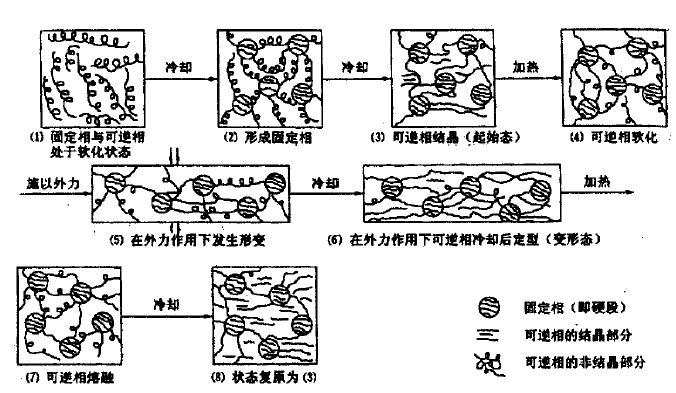
\includegraphics[width=0.75\textwidth]{figures/figure1}
 % \caption[这里的文字将会显示在 listoffigure 中]{这里的文字将会显示在正文中}
 \caption{热塑性形状记忆聚氨酯的形状记忆机理示意图}\label{fig:diagram}
\end{figure}


\subsection{形状记忆聚氨酯的研究进展}
%\label{sec:requirements}
首例SMPU是日本Mitsubishi公司开发成功的……。

\subsection{水系聚氨酯及聚氨酯整理剂}

水系聚氨酯的形态对其流动性,成膜性及加工织物的性能有重要影响,一般分为三种类型\cite{Jiang2005Size} ,如表 \ref{tab:category}所示。

\begin{table}[hbt]
  \centering
  \caption{水系聚氨酯分类} \label{tab:category}
  \begin{tabular*}{0.9\textwidth}{@{\extracolsep{\fill}}cccc}
  \toprule
    类别			&水溶型		&胶体分散型		&乳液型 \\
  \midrule
    状态			&溶解$\sim$胶束	&分散		&白浊 \\
    外观			&水溶型		&胶体分散型		&乳液型 \\
    粒径$/\mu m$	&$<0.001$		&$0.001-0.1$		&$>0.1$ \\
    重均分子量	&$1000\sim 10000$	&数千$\sim 20$万 &$>5000$ \\
  \bottomrule
  \end{tabular*}
\end{table}

\subsubsection{四级节标题}

根据需要,也可设四级节标题。

由于它们对纤维织物的浸透性和亲和性不同,因此在纺织品染整加工中的用途也有差别,其中以水溶型和乳液型产品较为常用。另外,水系聚氨酯又有反应性和非反应性之分。虽然它们的共同特点是分子结构中不含异氰酸酯基,但前者是用封闭剂将异氰酸酯基暂时封闭,在纺织品整理时复出。相互交联反应形成三维网状结构而固着在织物表面。
……


\section{常见问题和疑难解答}

如果您遇到\href{https://bithesis.bitnp.net/faq/char-missing.html}{生僻字无法显示}、
\href{https://bithesis.bitnp.net/faq/enumitem-nosep.html}{列表项间距过大}、
\href{https://bithesis.bitnp.net/faq/longtable.html}{三线表需要跨页}等问题,
请参考\textcolor{magenta}{\href{https://bithesis.bitnp.net/faq/}{在线文档的「疑难杂症」部分}}。

%%
% BIThesis 研究生学位论文模板 The BIThesis Template for Graduate Thesis
% This file has no copyright assigned and is placed in the Public Domain.
%%

\chapter{具体研究内容}

具体研究内容是学位论文的主要部分,是研究结果及其依据的具体表述,是研究能力的集中体现,一般应包括第2章、第3章至结论前一章。具体研究内容应该结构合理,层次清楚,重点突出,文字简练、通顺。可包括以下各方面:研究对象、研究方法、仪器设备、材料原料、实验和观测结果、理论推导、计算方法和编程原理、数据资料和经过加工整理的图表、理论分析、形成的论点和导出的结论等。具体研究内容各章后可有一节“本章小结”(必要时)。

\begin{them}[留数定理]
\label{thm:res}
  假设$U$是复平面上的一个单连通开子集,$a_1,\ldots,a_n$是复平面上有限个点,$f$是定义在$U\backslash \{a_1,\ldots,a_n\}$上的全纯函数,
  如果$\gamma$是一条把$a_1,\ldots,a_n$包围起来的可求长曲线,但不经过任何一个$a_k$,并且其起点与终点重合,那么:
  \begin{equation}
    \label{eq:res}
    \ointop_{\gamma}f(z)\,\mathrm{d}z = 2\pi\mathbf{i}\sum^n_{k=1}\mathrm{I}(\gamma,a_k)\mathrm{Res}(f,a_k)
  \end{equation}

  如果$\gamma$是若尔当曲线,那么$\mathrm{I}(\gamma, a_k)=1$,因此:
  \begin{equation}
    \label{eq:resthm}
    \ointop_{\gamma}f(z)\,\mathrm{d}z = 2\pi\mathbf{i}\sum^n_{k=1}\mathrm{Res}(f,a_k)
  \end{equation}

  在这里,$\mathrm{Res}(f, a_k)$表示$f$在点$a_k$的留数,$\mathrm{I}(\gamma,a_k)$表示$\gamma$关于点$a_k$的卷绕数。
  卷绕数是一个整数,它描述了曲线$\gamma$绕过点$a_k$的次数。如果$\gamma$依逆时针方向绕着$a_k$移动,卷绕数就是一个正数,
  如果$\gamma$根本不绕过$a_k$,卷绕数就是零。
\end{them}

\begin{proof}
  首先,由……

  其次,……

  所以,由\autoref{thm:res}可知……
  \qedhere
\end{proof}

\textit{有关公式与上下文间距的一些注意事项:请保证源码中的公式的环境(如}
\\ \verb|\begin{equation}|
  \textit{)与上一段落不要有空行。否则,公式和上文段落之间会有额外的空白。}


\backmatter

% 结论
%%
% BIThesis 读书报告模板 —— 使用 XeLaTeX 编译 The BIThesis Template for Reading Report
% This file has no copyright assigned and is placed in the Public Domain.
%% 

\begin{conclusion}
  % 结论部分尽量不使用 \subsection 二级标题,只使用 \section 一级标题

  % 这里插入一个参考文献,仅作参考
  本文结论……\cite{张伯伟2002全唐五代诗格会考}。

  \textcolor{blue}{结论作为正文的最后部分单独排写,但不加章号。阅后删除此段。}

  \textcolor{blue}{结论正文样式与文章正文相同:宋体、小四;行距:22磅;间距段前段后均为0行。阅后删除此段。}
\end{conclusion}

% 参考文献
%%
% BIThesis 读书报告模板 —— 使用 XeLaTeX 编译 The BIThesis Template for Reading Report
% This file has no copyright assigned and is placed in the Public Domain.
%%

\begin{bibprint}

% \printbibliography[heading=none]
% 正式使用时,请启用上方语句以输出所有的参考文献,并删除/注释下方示例内容。
% 删除后仍可参考 https://bithesis.bitnp.net/faq/bib-entry.html 的在线版本。

% -------------------------------- 示例内容(正式使用时请删除) ------------------------------------- %

% 抑制多次调用 \printbibliography 的 warning,只有示例代码会需要此语句。
\BiblatexSplitbibDefernumbersWarningOff

\textcolor{blue}{参考文献书写规范}

\textcolor{blue}{参考国家标准《信息与文献参考文献著录规则》【GB/T 7714—2015】,参考文献书写规范如下:}

\textcolor{blue}{\textbf{1. 文献类型和标识代码}}

\textcolor{blue}{普通图书:M}\qquad\textcolor{blue}{会议录:C}\qquad\textcolor{blue}{汇编:G}\qquad\textcolor{blue}{报纸:N}

\textcolor{blue}{期刊:J}\qquad\textcolor{blue}{学位论文:D}\qquad\textcolor{blue}{报告:R}\qquad\textcolor{blue}{标准:S}

\textcolor{blue}{专利:P}\qquad\textcolor{blue}{数据库:DB}\qquad\textcolor{blue}{计算机程序:CP}\qquad\textcolor{blue}{电子公告:EB}

\textcolor{blue}{档案:A}\qquad\textcolor{blue}{舆图:CM}\qquad\textcolor{blue}{数据集:DS}\qquad\textcolor{blue}{其他:Z}

\textcolor{blue}{\textbf{2. 不同类别文献书写规范要求}}

\textcolor{blue}{\textbf{期刊}}

\noindent\textcolor{blue}{[序号] 主要责任者. 文献题名[J]. 刊名, 出版年份, 卷号(期号): 起止页码. }
\cite{yuFeiJiZongTiDuoXueKeSheJiYouHuaDeXianZhuangYuFaZhanFangXiang2008, Hajela2012Application}

\printbibliography [type=article,heading=none]

\textcolor{blue}{\textbf{普通图书}}

\noindent\textcolor{blue}{[序号] 主要责任者. 文献题名[M]. 出版地: 出版者, 出版年: 起止页码. }
\cite{张伯伟2002全唐五代诗格会考, OBRIEN1994Aircraft}

\printbibliography [keyword={book},heading=none]

\textcolor{blue}{\textbf{会议论文集}}

\noindent\textcolor{blue}{[序号] 主要责任者.题名:其他题名信息[C]. 出版地: 出版者, 出版年. }
\cite{雷光春2012}

\printbibliography [type=proceedings,heading=none]

\textcolor{blue}{\textbf{专著中析出的文献}}

\noindent\textcolor{blue}{[序号] 析出文献主要责任者. 析出题名[M]//专著主要责任者. 专著题名. 出版地: 出版者, 出版年: 起止页码. }
\cite{白书农}

\printbibliography [type=inbook,heading=none]

\textcolor{blue}{\textbf{学位论文}}

\noindent\textcolor{blue}{[序号] 主要责任者. 文献题名[D]. 保存地: 保存单位, 年份. }
\cite{zhanghesheng, Sobieski}

\printbibliography [keyword={thesis},heading=none]

\textcolor{blue}{\textbf{报告}}

\noindent\textcolor{blue}{[序号] 主要责任者. 文献题名[R]. 报告地: 报告会主办单位, 年份. }
\cite{fengxiqiao, Sobieszczanski}

\printbibliography [keyword={techreport},heading=none]

\textcolor{blue}{\textbf{专利文献}}

\noindent\textcolor{blue}{[序号] 专利所有者. 专利题名:专利号[P]. 公告日期或公开日期[引用日期]. 获取和访问路径. 数字对象唯一标识符.}
\cite{jiangxizhou}

\printbibliography [type=patent,heading=none]

\textcolor{blue}{\textbf{国际、国家标准}}

\noindent\textcolor{blue}{[序号] 主要责任人. 题名: 其他题名信息[S]. 出版地: 出版者, 出版年: 引文页码.}
\cite{GB/T3792.4-2009}

\printbibliography [keyword={standard},heading=none]

\textcolor{blue}{\textbf{报纸文章}}

\noindent\textcolor{blue}{[序号] 主要责任者. 文献题名[N]. 报纸名, 年(期): 页码. }
\cite{xiexide}

\printbibliography [keyword={newspaper},heading=none]

\textcolor{blue}{\textbf{电子文献}}

\noindent\textcolor{blue}{[序号] 主要责任者. 电子文献题名[文献类型/载体类型]. (发表或更新日期) [引用日期]. 获取和访问路径. 数字对象唯一标识符. }
\cite{yaoboyuan}

\printbibliography [keyword={online},heading=none]

\textcolor{blue}{关于参考文献的未尽事项可参考国家标准《信息与文献参考文献著录规则》(GB/T 7714—2015)}

\end{bibprint}


% 附录
%%
% BIThesis 研究生学位论文模板 The BIThesis Template for Graduate Thesis
% This file has no copyright assigned and is placed in the Public Domain.
%%

\begin{appendices}
  \chapter{费马大定理的证明}
  关于此,我确信已发现了一种美妙的证法,可惜这里空白的地方太小,写不下。

  \chapter{Maxwell Equations}
  因为在柱坐标系下,$\overline{\overline\mu}$是对角的,所以Maxwell方程组中电场$\bf
  E$的旋度

  所以$\bf H$的各个分量可以写为:
  \begin{subequations}
    \begin{eqnarray}
      H_r=\frac{1}{\mathbf{i}\omega\mu_r}\frac{1}{r}\frac{\partial
        E_z}{\partial\theta } \\
      H_\theta=-\frac{1}{\mathbf{i}\omega\mu_\theta}\frac{\partial E_z}{\partial r}
    \end{eqnarray}
  \end{subequations}

  同样地,在柱坐标系下,$\overline{\overline\epsilon}$是对角的,所以Maxwell方程组中磁场$\bf
  H$的旋度
  \begin{subequations}
    \begin{eqnarray}
      &&\nabla\times{\bf H}=-\mathbf{i}\omega{\bf D}\\
      &&\left[\frac{1}{r}\frac{\partial}{\partial
          r}(rH_\theta)-\frac{1}{r}\frac{\partial
          H_r}{\partial\theta}\right]{\hat{\bf
          z}}=-\mathbf{i}\omega{\overline{\overline\epsilon}}{\bf
        E}=-\mathbf{i}\omega\epsilon_zE_z{\hat{\bf z}} \\
      &&\frac{1}{r}\frac{\partial}{\partial
        r}(rH_\theta)-\frac{1}{r}\frac{\partial
        H_r}{\partial\theta}=-\mathbf{i}\omega\epsilon_zE_z
    \end{eqnarray}
  \end{subequations}

  由此我们可以得到关于$E_z$的波函数方程:
  \begin{eqnarray}
    \frac{1}{\mu_\theta\epsilon_z}\frac{1}{r}\frac{\partial}{\partial r}
    \left(r\frac{\partial E_z}{\partial r}\right)+
    \frac{1}{\mu_r\epsilon_z}\frac{1}{r^2}\frac{\partial^2E_z}{\partial\theta^2}
    +\omega^2 E_z=0
  \end{eqnarray}

  \chapter{要求}

  \textcolor{blue}{
  有些材料编入文章主体会有损于编排的条理性和逻辑性,或有碍于文章结构的紧凑和突出主题思想等,这些材料可作为附录另页排在参考文献之后,也可以单编成册。下列内容可作为附录:
  }
  \begin{enumerate}
    \item \textcolor{blue}{为了整篇论文材料的完整,但编入正文有损于编排的条理性和逻辑性的材料,这一类材料包括比正文更为详尽的信息、研究方法和技术等更深入的叙述,以及建议可阅读的参考文献题录和对了解正文内容有用的补充信息等;}
    \item \textcolor{blue}{ 由于篇幅过大或取材的复制资料不便于编入正文的材料; }
    \item \textcolor{blue}{ 不便于编入正文的罕见珍贵资料; }
    \item \textcolor{blue}{ 一般读者无须阅读,但对本专业同行有参考价值的资料; }
    \item \textcolor{blue}{ 某些重要的原始数据、推导、计算程序、框图、结构图、注释、统计表、计算机打印输出件等; }
  \end{enumerate}

  \section{一级标题}
  \subsection{二级标题}
\end{appendices}


% 个人成果
%%
% BIThesis 研究生学位论文模板 The BIThesis Template for Graduate Thesis
% This file has no copyright assigned and is placed in the Public Domain.
%%

% ==== 攻读学位期间发表论文与研究成果清单 ====
% 1. 在 `../reference/pub.bib` 中添加数据。
% 2. 在本文件下方 `\addpubs` 添加该文献(参考下方示例)。

% **注意:如果发现渲染出来的文献编号不正确,请同时使用以下两个方式解决:**
% 1. 请清除缓存重新编译,比如`latexmk -gg`,详见 https://bithesis.bitnp.net/faq/clean.html 。
% 2. 请确保无编译错误。

\begin{publications}

  % **默认情况下,这里的内容将按照学校要求,以发表时间排序。**
  % - 如果想要按照引用顺序排序,可在`main.tex`设置`publications/sorting = false`。
  % - 如果想要微调,详见 https://bithesis.bitnp.net/faq/bib-sort.html#sortkey 。
  % 更多信息请参考「bithesis.pdf」手册。
  \addpubs{myCiteKey,myCiteKey2,dummy:1,dummy:2}

  % 主要针对硕士生
  \printbibliography[heading=none,category=mypub,resetnumbers=true]

  % 如果想要分为多个列表,可以使用以下的命令。
  % 主要针对博士生。
  % \pubsection{文章}
  % \printbibliography[heading=none,type=article,category=mypub,resetnumbers=true]{}
  %
  % \pubsection{一些书}
  % \printbibliography[heading=none,type=book,category=mypub,resetnumbers=true,notkeyword=dummy]
  %
  % \pubsection{另一些书}
  % \printbibliography[heading=none,type=book,category=mypub,keyword=dummy,resetnumbers=true]
  %
  % 关于 \printbibliography 的筛选参数:
  % 0. 请保留“category=mypub”。(这样只列出成果,不列出正文参考文献。)
  % 1. 设置“type=…”,每次只输出某一类型。
  % 2. 若需继续细分,请在 pub.bib 的条目里记录“keywords = {…, …}”,然后在此用“keyword=…”筛选。
  % 3. 如果还有要求,可用notkeyword、subtype等筛选方法,请参考 biblatex 手册。

  % 如果想绕过 pub.bib 直接记录项目(例如获奖),请参考以下内容,
  % 定义一个能和 \printbibliography 共存的列表。
  % https://bithesis.bitnp.net/faq/pub-manual.html
  % \zihao{5} % 字号改为五号
  % \renewcommand{\labelenumi}{[\theenumi]} % 编号改用中括号
  %
  % \begin{enumerate}[nosep, leftmargin=4ex-2pt, labelsep=1ex]
  %   \setcounter{enumi}{4} % 下一项为 5。
  %   \item 于《新青年》发表论文一篇,本人第一作者。
  %   \item 于\textit{La Jeunesse}发表论文一篇,导师第一作者,本人第二作者。
  % \end{enumerate}
\end{publications}


% 致谢
%%
% BIThesis 研究生学位论文模板 The BIThesis Template for Graduate Thesis
% This file has no copyright assigned and is placed in the Public Domain.
%%

\begin{acknowledgements}

本论文的工作是在导师……。

\textcolor{blue}{
  致谢是对下列方面致谢:资助和支持者;协助完成研究工作和提供便利条件者;在研究工作中提出建议和提供帮助者;给予转载和引用权的资料、图片、文献、研究思想和设想的所有者;其他应感谢者。致谢语言要诚恳、恰当、简短。
}

\end{acknowledgements}

% 个人简介(仅博士生需要此项)
%%
% BIThesis 研究生学位论文模板 The BIThesis Template for Graduate Thesis
% This file has no copyright assigned and is placed in the Public Domain.
%%

\begin{resume}

本人…。

\textcolor{blue}{
  硕士学位论文不必提供作者简介。博士学位论文应该提供作者简介,主要包括:姓名、性别、出生年月、民族、出生地;简要学历、工作经历(职务);攻读学位期间取得的其他研究成果或奖励。
}

\end{resume}


% 在全文最后,博士附《博士学位论文答辩表》前2页决议含签字的扫描版,硕士不用附。
% 建议用 Word 模板填写该表,扫描后拼接 PDF。

\end{document}
